\documentclass{article}

\usepackage{titling}
\usepackage{graphicx}
\usepackage{graphicx}
\usepackage[export]{adjustbox}

\title{Programación Concurrente}
\author{Tomas Sarquis}
\date{Julio 2020}

\begin{document}
    %%%%%%%%%%%%%%%%%%%%%%%%%%%%%%%%%%%%%%%%%%%%%%%%%%%%%%%%%%%%%%%%%%%%%%%%%%%%%%%%%%%%%%%%
    \begin{titlingpage}
        \maketitle
        \topskip0pt
        \vspace*{\fill}
        El presente documento detalla la realización del \textbf{trabajo práctico número 3} 
        de la asignatura \textbf{programación concurrente}, correspondiente al año \textbf{2019}
        por el alumno Tomas Sarquis, matrícula 39884977
        \vspace*{\fill}
    \end{titlingpage}
    %%%%%%%%%%%%%%%%%%%%%%%%%%%%%%%%%%%%%%%%%%%%%%%%%%%%%%%%%%%%%%%%%%%%%%%%%%%%%%%%%%%%%%%%
    \section{Enunciado}
    \begin{flushleft}
        Se debe implementar un simulador de un procesador con dos núcleos. A partir de la red de
        Petri de la \emph{figura 1}, la cual representa a un procesador mono núcleo, se deberá 
        extender la misma a una red que modele un procesador con dos núcleos. Además, se debe
        implementar una política que resuelva los conflictos que se generan con las transiciones
        que alimentan los buffers de los núcleos.
    \end{flushleft}
    \begin{figure}[h]
        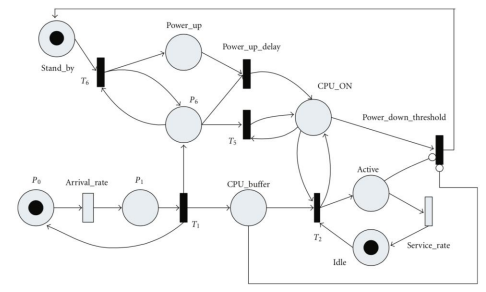
\includegraphics[width=0.9\textwidth, center]{rdp_enun.png}
        \caption{red de Petri mono núcleo}
    \end{figure}
    %%%%%%%%%%%%%%%%%%%%%%%%%%%%%%%%%%%%%%%%%%%%%%%%%%%%%%%%%%%%%%%%%%%%%%%%%%%%%%%%%%%%%%%%
    \section{Implementación y resultados}
    %%%%%%%%%%%%%%%%%%%%%%%%%%%%%%%%%%%%%%%%%%%%%%%%%%%%%%%%%%%%%%%%%%%%%%%%%%%%%%%%%%%%%%%%
    \subsection{Red de Petri}
    \begin{flushleft}
        En la \emph{figura 2} se observa cómo fue modelada la red de Petri de acuerdo al enunciado. \par
        La red de Petri modelada cuenta con:
    \end{flushleft}
    \begin{itemize}
        \item 16 plazas
        \item 15 transiciones
    \end{itemize}
    \begin{figure}[t]
        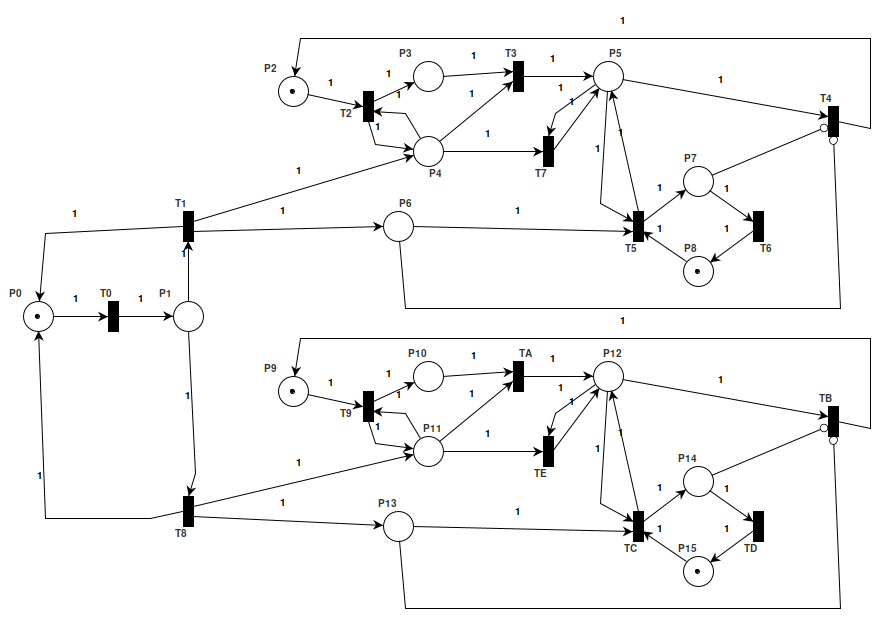
\includegraphics[width=0.9\textwidth, center]{rdp.png}
        \caption{red de Petri doble núcleo}
    \end{figure}   
    %%%%%%%%%%%%%%%%%%%%%%%%%%%%%%%%%%%%%%%%%%%%%%%%%%%%%%%%%%%%%%%%%%%%%%%%%%%%%%%%%%%%%%%%
    \subsection{Hilos}
    \begin{flushleft}
        Teniendo en cuenta la red de la \emph{figura 2}, lo siguiente es pensar cuántos hilos
        serán los encargados de ejecutarse el programa. \\
        Luego de realizar un análisis, se llegó a la conclusión de que en la red deben trabajar
        \textbf{7 hilos} en forma concurrente. Estos hilos son llamados:
        \begin{itemize}
            \item ProcessGenerator
            \item CPUPower x 2
            \item CPUProcessing x 2
            \item CPUGarbageCollector x 2
        \end{itemize}
        \textbf{ProcessGenerator:} Encargado de generar los procesos comúnes a ambos CPUs. 
        Dispara las transiciones 0, 1 y 8. \newline \newline
        \textbf{CPUPower:} Maneja el encendido/apagado de cada CPU. Dispara las transiciones
        2, 3 y 4 o 9, A y B. \newline \newline
        \textbf{CPUProcessing:} Procesa las tareas de cada CPU. Dispara las transiciones
        2, 3 y 4 o 9, A y B. \newline \newline
        \textbf{CPUGarbageCollector:} Previene que la plaza número 4/11 no junte \emph{tokens}
        "basura". \newline \newline
    \end{flushleft}
    %%%%%%%%%%%%%%%%%%%%%%%%%%%%%%%%%%%%%%%%%%%%%%%%%%%%%%%%%%%%%%%%%%%%%%%%%%%%%%%%%%%%%%%%
    \subsection{Clases en Java}
    \begin{flushleft}
        El programa encargado de simular el sistema se desarrola en el lenguaje de programación
        \emph{Java}. A continuación, se describen las clases, implementadas en dicho lenguaje,
        que modelan el programa:
        \begin{itemize}
            \item \textbf{Cola:} Colas (\emph{queues}), las cuales son usadas para que los
            hilos puedan dormir en caso que lo necesiten
            \item \textbf{Colors:} Clase sin funciones que contiene códigos de colores (para 
            loggear)
            \item \textbf{CPUGarbageCollector:} Modelo del hilo CPUGarbageCollector anteriormente
            descrito
            \item \textbf{CPU:} Modela un CPU. Clase encargada de "comunicar" los hilos Generator,
            Processing y GarbageCollector
            \item \textbf{CPUPower:} Modelo del hilo CPUPower anteriormente descrito
            \item \textbf{CPUProcessing:} Modelo del hilo CPUProcessing anteriormente descrito
            \item \textbf{InvarianteTest:} Implementación de un test de t-invariantes
            \item \textbf{Main:} Clase principal y ejecutable
            \item \textbf{Monitor:} Encargada de administrar los tiempos y el uso de la red de 
            Petri
            \item \textbf{Politica:} A la hora de despertar un hilo, la politica es quien decide
            a cuál hacerlo
            \item \textbf{ProcessBuffer:} Modelo de un buffer en el cuál se depositan Process
            \item \textbf{ProcessGenerator:} Modelo del hilo ProcessGenerator anteriormente
            descrito
            \item \textbf{Process:} Clase que simula un proceso de CPU. Dichos Process van a
            parar a un ProcessBuffer
            \item \textbf{RedDePetri:} Implementación de la red de Petri
        \end{itemize}
        Para información más detallada acerca de las clases y sus funciones, se puede consultar
        la documentación\footnote{La documentación se encuentra en el archivo \emph{html}
        "documentacion/html/index.html"} hecha por \emph{Doxygen}\footnote{www.doxygen.nl}.
    \end{flushleft}
    %%%%%%%%%%%%%%%%%%%%%%%%%%%%%%%%%%%%%%%%%%%%%%%%%%%%%%%%%%%%%%%%%%%%%%%%%%%%%%%%%%%%%%%%
    \subsection{Invariantes}
    \begin{flushleft}
        Sabemos que una de las maneras de chequear que la red (y nuestro programa) funciona 
        de forma correcta, es analizando las invariantes. Estas son, las \textbf{t-invariantes}
        y las \textbf{p-invariantes}. \\
        Para el análisis, se usó la herramienta Pipe\footnote{http://pipe2.sourceforge.net/}.
        Los resultados fueron los siguientes: \newline \newline
        \textbf{P-Invariantes:} \\
        \begin{figure}[h]
            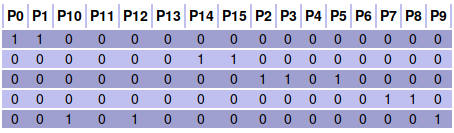
\includegraphics[width=0.7\textwidth, center]{p-invariante.png}
            \caption{análisis de P-Invariantes en Pipe}
        \end{figure}
        La \emph{figura 3} nos enseña qué plazas están relacionadas mediante una invariante de
        plazas. Esta relación indica que la suma de los \emph{tokens} en dichas plazas, en cada
        relación, sea siempre unitaria. Estos es: \newline \newline
        $M(P0) + M(P1) = 1$ \newline \newline
        $M(P14) + M(P15) = 1$ \newline \newline
        $M(P2) + M(P3) + M(P5) = 1$ \newline \newline
        $M(P10) + M(P12) + M(P9) = 1$ \newline \newline
        Para comprobar que lo anterior se cumpla siempre, la clase \emph{RedDePetri} hace un 
        chequeo cada vez que se dispara una transición. El método de la clase que hace dicho
        chequeo se llama \emph{isPInvariantesCorrecto}. \newline \newline
        \textbf{T-Invariantes:} \newline \newline
        De la misma forma, podemos observar en la \emph{figura 4} las invariantes de transición
        que existen en nuestro sistema. \\
        \begin{figure}[h]
            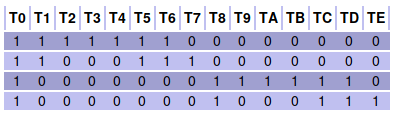
\includegraphics[width=0.7\textwidth, center]{t-invariante.png}
            \caption{análisis de T-Invariantes en Pipe}
        \end{figure}   
        Anteriormente se mencionó la clase \emph{InvarianteTest}. Esta clase es la encargada
        de chequear, una vez finalizada la ejecución, que el orden de los disparos (de las 
        transiciones) sea el correcto. \\
        Para esto, la clase \emph{Main} se encarga de grabar todas las transiciones (en orden) 
        que han sido disparadas en un archivo\footnote{src/T-Invariantes.txt} de texto. Luego, la
        clase \emph{InvarianteTest} usa esa información para, mediante un algoritmo de remplazo,
        ir eliminando las coincidencias (o \emph{matches}) entre el \emph{log} de transiciones y
        las invariantes. Si el sistema funciona correctamente, deben quedar eliminadas todas las
        transiciones. De lo contrario, existen errores, que son escritos en otro 
        archivo\footnote{src/T-InvariantesErr.txt} de texto. \newline \newline
        \textbf{Resultados:} \newline \newline
        Al finalizar una ejecución, se loggea el estado de los análisis de invariantes. Un ejemplo
        se puede ver en la \emph{figura 5}.
        \begin{figure}[h]
            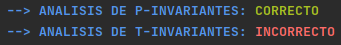
\includegraphics[width=0.5\textwidth, center]{analisis-invariantes-ej.png}
            \caption{ejemplo del análisis de invariantes de una ejecución}
        \end{figure}

    \end{flushleft}
\end{document}